%
%  CfA Proposal Template for time at FLWO/MMT/Magellan
%
%  Use this template for all observing proposals.
%  No style file is required.
%
%  Version 1.1    8 October 2010
%  Changed topmargin from 0.25in to 0.5in (DJM 2010-10-08)
%
%  Version 1.2    12 April 2016
%  Changed topmargin from 0.5in to 1.0in (DJM 2010-10-08)
%
%%%  For information on CfA observing facilities please visit
%    the CfA TAC web page:
%
%%%  http://www.cfa.harvard.edu/~kenyon/TAC/
%
%%%%%%%%%%%%%%%%%%%%%%%%%%%%%%%%%%%%%%%%%%%%%%%%%%%%%%%%%%%%%%%%%%%%%%%%
%
%  The template begins here.  The font must be 12 point, the vertical
%  line spacing must be 12.5 point, and the margins must be at least
%  1-inch on all sides.
%
%  Do not override these limits
%
%  To produce a postscript file with better computer viewable fonts,
%  please use dvips -Ppdf -o file.ps file.dvi
%
\documentclass[12pt]{article}
\usepackage{graphicx}
\usepackage{amssymb}

\pdfpagewidth 8.5in
\pdfpageheight 11in

\linespread{1.042}
\normalsize
\textwidth=6.5in
\textheight=9.0in
\topmargin=0.0in
\oddsidemargin=0.0in
\evensidemargin=0.0in
\pagenumbering{arabic}
\usepackage[top=1.in, bottom=1.in, left=1.in, right=1.in, bindingoffset=0.0in]{geometry}
\usepackage{parskip}
\setlength{\parindent}{0cm}
\renewcommand{\floatpagefraction}{0.9}

\usepackage{cfa}

\begin{document}
%%% The proposal consists of these sections:
%
%   Scientific justification & Experimental design: up to 2 pages of text
%   References, Figures, target list, and publications: up to 2 pages
%
% \vspace{-1cm}
\section*{Scientific Justification}\vskip-0.2in

% Describe the background and goals for your project.

% <<<<<<< HEAD
% Clumpiness of matter on small scales remains one of the most pressing questions in cosmology (Bullock \& Boylan-Kolchin 2017).
% In the $\Lambda$CDM model, clumps of dark matter with no baryons are expected to exist down to mass scales of at least $10^{6}\rm\,M_\odot$ (Springel et al. 2008), while alternative models have a higher cut-off in the matter power spectrum (e.g., Bode et al. 2001, Hu et al. 2000).
% Cold stellar streams, remnants of disrupted globular clusters discovered in the Galactic halo (Grillmair \& Carlin 2016), are sensitive to the underlying acceleration field (Bonaca \& Hogg 2018).
% An encounter with a dark matter subhalo would perturb the orderly structure of the stellar stream, produce density variations along the stream (e.g., Carlberg 2012), and, depending on geometry, possibly also fold a part of the stream (e.g., Yoon et al. 2011).
% We propose to obtain high-resolution spectra, and thus map the full phase-space distribution of the GD-1 stellar stream, a stream with the strongest indications of perturbation by dark matter substructure.
% =======
Clumpiness of matter on small scales remains one of the most pressing questions in cosmology and galaxy formation (Bullock \& Boylan-Kolchin 2017).
In the $\Lambda$CDM model, clumps of dark matter with no baryons are expected to exist with masses as low as $10^{6}\rm\,M_\odot$ (Springel et al. 2008), while alternative models have a higher cut-off in the matter power spectrum (e.g., Bode et al. 2001, Hu et al. 2000).
Cold stellar streams --- remnants of disrupted globular clusters discovered in the Galactic halo (Grillmair \& Carlin 2016) --- are unique and powerful tools to study the properties of mass and dark matter within the Galaxy (e.g., Bonaca \& Hogg 2018).
For example, an encounter between a stellar stream and a dark matter subhalo perturbs the orderly structure of the stellar stream, produces density variations along the stream (e.g., Carlberg 2012), and, depending on geometry, possibly also folds a part of the stream (e.g., Yoon et al. 2011).
Signatures of such interactions in any of the known Milky Way stellar streams would provide critical tests of dark matter theories.
We propose to obtain high-resolution spectra to combine with kinematic data from the Gaia mission and thus map the full (6D) phase-space distribution of the GD-1 stellar stream, a nearby, dense stellar stream that shows possible signatures of subhalo perturbations.

{\bf GD-1 -- a halo stream with signatures of perturbation:}
The GD-1 stellar stream was discovered using photometry from the Sloan Digital Sky Survey (SDSS; Grillmair \& Dionatos 2006),
% and was later characterized using a combination of SDSS spectroscopic radial velocities and mean proper motions (Koposov et al. 2010).
% The stream appears to be on a retrograde orbit with respect to the Galactic disk, and, because of its relative proximity ($\sim 10~\textrm{kpc}$), appears as a significant over-density of old, metal-poor main-sequence turnoff stars.
and, in combination with handful of radial velocities for red giant star members, has been used to measure the mass and shape of the large-scale mass distribution within the Galaxy (Koposov et al. 2010; Bovy et al. 2016).
Using deeper photometry, de Boer at al. (2018) noted density variations along the stream and possible deviations of the main stream track that are not expected from simple models of the stream formation.
However, photometric studies alone suffer from significant contamination from background and foreground stars.
As an alternative approach to selecting likely GD-1 members, we mapped the stream additionally selecting members using the exquisite proper motions from the \textit{Gaia} mission (Figure~1, Price-Whelan \& Bonaca 2018).
This relatively contamination-free view of the stream reveals two significant gaps along the stream, one of which is associated with a spur of member stars parallel to the main stream, but offset from it by $\sim1^\circ$.
Such morphology can result from a stream interaction with a massive perturber (Figure~2).

% With this relatively contamination-free view of the stream and map of individual stream members, it is clear that (1) the stream extends at least $30^\circ$ beyond the previously seen end, and (2) that there is indeed interesting structure in the density distribution along the stream.
% In particular, ... under-densities... spur...blob...


% - discovered
% - density variations carlberg + later
% - Gaia and new era of stream kinematics, summarize our paper
% [Subhalo interactions with streams can leave gaps...Yoon, Erkal, etc.]

% - figure 1: map from paper, inset w transparent map, solid top priority -- getting most, typically 10 in dense Hectochelle fields, 5 in sparse, and expecting only a couple of Milky Way field contaminants

{\bf Hectochelle spectroscopy as the missing piece of the puzzle:}
Even after a selection based both on photometry and proper motions, some Milky Way contamination remains in the GD-1 sample (e.g., stars at $|\phi_2|>2^\circ$ in Figure~1).
We propose obtaining Hectochelle spectroscopy of likely GD-1 members to further confirm their common origin.
These data will provide radial velocities, and distance estimates more accurate than the available parallaxes, thus completely mapping the phase space distribution of the debris.
We plan to survey the highly non-uniform region of the stream, focusing in particular on the gap in the stream and the spur beyond the stream.
Simulations of stream perturbations predict unique signatures in the 3D kinematic structure of the debris (e.g., Figure~2, see also Erkal \& Belokurov 2015), so the proposed data will be able to rule on the interaction origin of features observed in the GD-1 stream and provide a critical test of the $\Lambda$CDM paradigm.

% [But, other things can cause gaps too (epicyclic over-densities, progenitor disruption)]
% - in the interaction scenario (Figure~2), we expect velocity offsets between the stream and the spur, corresponding to an energy imparted by the perturber, and potentially constraining its mass.
% [Need 3D pos and vel to study velocity distribution along stream / energy offsets to know for sure]

% Radial velocities of the stream members are crucial for accurate gravitational potential recovery (Figure~2).
% Here \textbf{we propose to measure radial velocities for 150 stars along the NGC~5466 and Styx streams with MMT/Hectochelle}.
% The Hectochelle field-of-view is well matched to the streams' widths, and its sensitivity allows efficient mapping of the entire streams.
% Combined with the data already at hand for Pal~5 and GD-1 streams, using these new measurements within our modeling framework will provide significantly improved constraints on the distribution of dark matter within 50~kpc.

\pagebreak
\section*{Experimental Design}\vskip-0.2in

% Describe the proposed observations and the targets.

\noindent{\bf Observing Strategy:}
We will use MMT/Hectochelle spectrograph to measure radial velocities of stars in the GD-1 stream.
Prior to the second data release from the \emph{Gaia} mission, spectroscopic follow-up of diffuse, distant structures such as cold stellar streams was plagued by contamination from the much more numerous nearby dwarf stars.
However, a selection on small \emph{Gaia} parallaxes immediately removes most of the contamination from the target list.
Additionally, GD-1 is a particularly opportune observing target as it is on a retrograde orbit, so its members stand out from the field Milky Way population in proper motions as well (Figure~3, left).
It is also fairly old, metal-poor and nearby, so its main sequence is well delineated from the Milky Way field in the color-magnitude diagram (Figure~3, center).
Pilot data taken in 2018B, courtesy of the H3 survey, indicate that targeting using both proper motions and photometry yields a very high success rate in identifying members of the GD-1 stream (Figure~3, right). 
% Both streams are photometrically detected in the SDSS, which we will use for spectroscopic targeting.
% Streams occupy a well defined region in the color-magnitude diagram (Figure~3, NGC~5466 on the left, and Styx in the middle), so target priorities will be assigned through matched filtering to reduce the contamination from the Milky Way field stars.
% We aim to identify $\sim150$ stream members, as our preliminary modeling shows that such a number of radial velocity measurements is sufficient to place accurate and tight constraints on the Galactic gravitational potential.
% This will also be comparable to the number of radial velocity measurements for Pal~5 and GD-1 streams.
% However, since the targeted streams are much more tenuous than either Pal~5 or GD-1 (Grillmair \& Johnson 2006), we require more pointings for a given limiting magnitude to identify the same number of members.
% These observations will break new ground in exploring kinematics of diffuse halo substructure, and will also guide our future campaigns aimed at kinematic profiling of all the cold streams in the Milky Way.

\noindent{\bf MMT/Hectochelle Spectroscopy:}
We will observe with MMT/Hectochelle using the 110\,$l$/mm grating and the `RV31' order-blocking filter over the wavelength range 5150--5300\,\AA, yielding $\sim$1.5~km\,s$^{-1}$ per resolution element.
The velocity precision achieved by the TDC Hectochelle pipeline and this setup under typical observing conditions is further improved to better than 1\,km/s.
The chosen wavelength region contains the Mgb triplet and an assortment of Fe~II lines, which will be used to measure chemical abundances with the Payne code (Ting et al. 2018).
We will assign membership probability of each target based on the Gaia proper motions, PanSTARRS photometry, measured radial velocity and metallicity.
Target selection based on proper motions is highly efficient, so there are on average $\sim10$ top priority targets per Hectochelle field.
We plan to dedicate additional $\sim40$ fibers to lower priority stars with similar proper motions, and $\sim150$ fibers to field halo stars (selected to have small parallax) in order to complement the H3 survey (PI Conroy) at fainter magnitudes.
The remaining $\sim40$ fibers will be used to estimate sky background throughout the field.

\noindent{\bf Proposal Time Request:}
To map the entire region of GD-1 with signatures of a potential perturbation (Figure~1), we require 13 Hectochelle pointings: 4 along the spur matched by 4 along the stream, and 3 along the gap.
Previous experience suggests that we can reach our targeted velocity uncertainty of $\lesssim$1 km/s in 2.5 hours for stars as faint as $g=20.5$.
Including overheads for field acquisition and calibration ($\sim$30 minutes per pointing), completing the observations of the planned 13 fields will therefore require $\sim$39 hours, or 4 nights.

{\par\bf R.A. range of principal targets (hours): }10 to 10:30
{\par\bf Dec. range of principal targets (degrees): }+35 to +45

\pagebreak

\begin{figure*}
\begin{center}
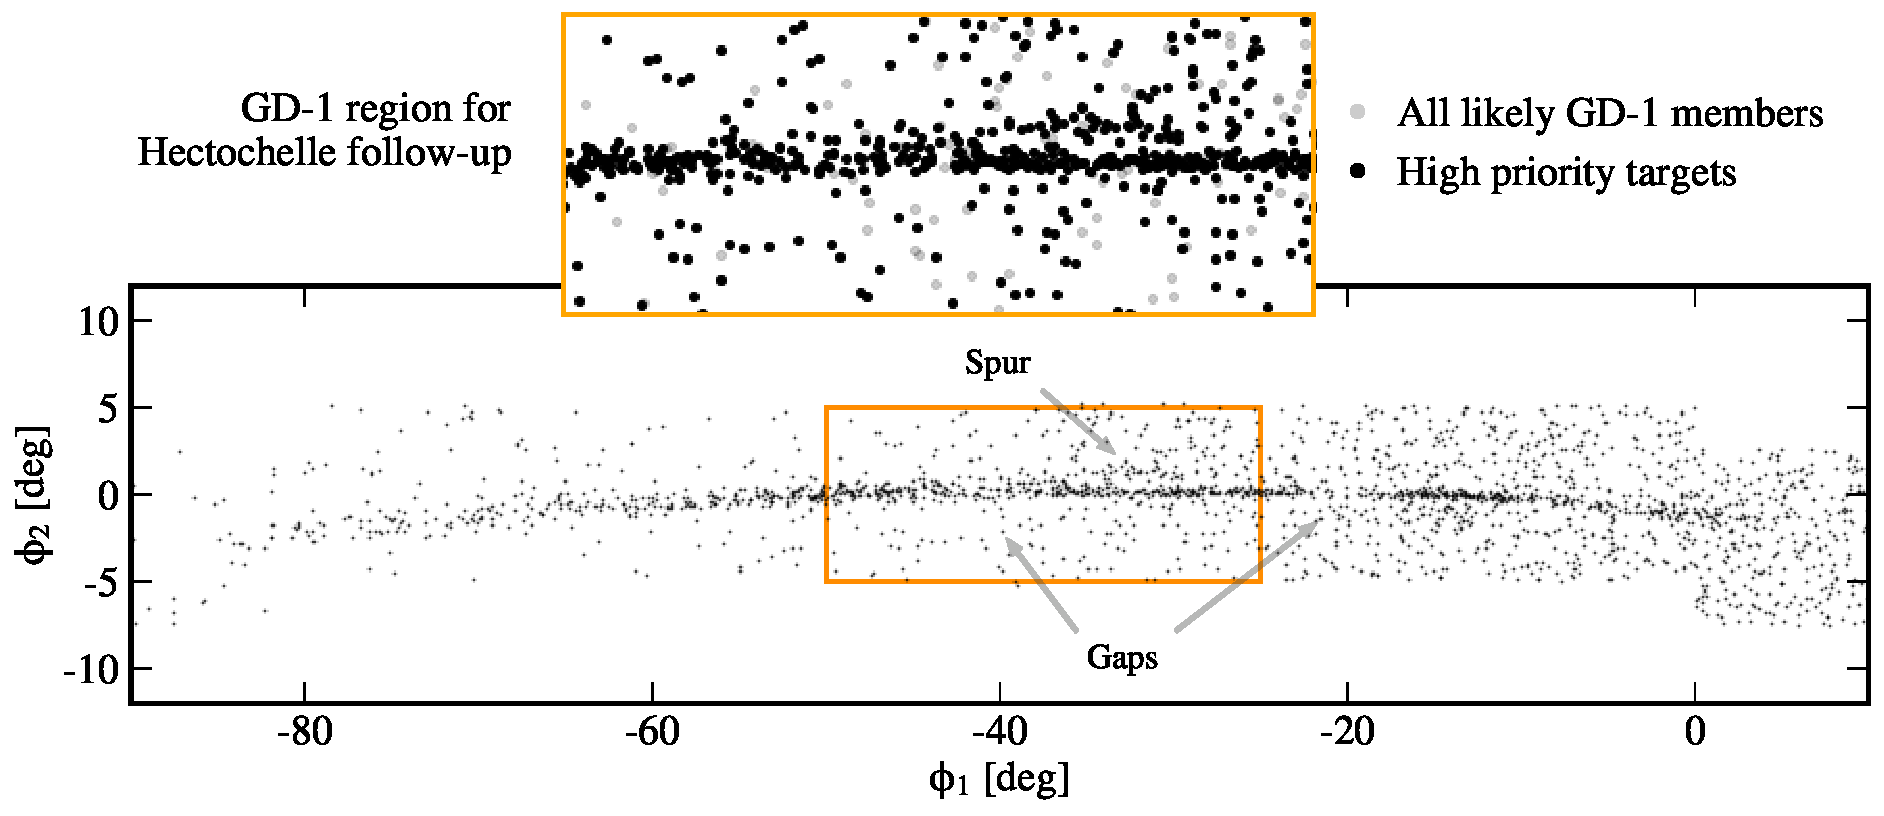
\includegraphics[width=1\textwidth]{../plots/prop_fig1.pdf}
\caption{\small On-sky positions of likely GD-1 members in the GD-1 coordinate system, selected using \emph{Gaia} proper motions and PanSTARRS photometry.
Inset shows the region with the unusual morphology of an underdensity along the stream (gap) and an overdensity of GD-1-like stars beyond the main stream (spur).
{\bf Proposed observations will result in the complete 6D phase-space coordinates for almost all of the likely GD-1 members}, illuminate the peculiar nature of the stream itself and inform on the clumpiness of matter on small scales.
% Stellar density map of the Milky Way halo, obtained by matched-filtering the SDSS photometric catalog, reveals a wealth of substructure (modified from Grillmair \& Carlin 2016).
% Previous follow-up campaigns have spectroscopically characterized more extended features, such as the Sagittarius stream or the Virgo Overdensity.
% However, the underlying gravitational potential is most exquisitely traced by the cold and narrow streams, and its accurate reconstruction requires dynamical information.
% {\bf We propose to measure radial velocities along the NGC~5466 tidal tails and the Styx stream, thus doubling the census of cold streams with kinematic constraints, and validating current constraints on the Galactic gravitational potential}.
}
\label{fig:fos}
\end{center}
\end{figure*}

\begin{figure*}\vskip-0.1in
\begin{center}
\includegraphics[width=0.5\textwidth]{../plots/prop_fig2a.pdf}
\hspace{0.2cm}
\includegraphics[width=0.43\textwidth]{../plots/prop_fig2b.pdf}
\caption{\small Idealized interaction of a stellar stream with a $5\cdot10^6\,\rm M_\odot$ perturber extends the stream in the direction of the closest encounter, $(x,y)=(0,-100\,\rm pc)$. 
Snapshots of the stream first extending, and then looping, are shown in the left panel, with darker colors corresponding to a longer time after the encounter.
Although the exact configuration depends on the viewing angle, {\bf loops of stream stars formed following a perturbation are in general both spatially and kinematically offset from the main stream} (right). 
Expected differences in radial velocity of a few km\,s$^{-1}$ are easily resolved using the Hectochelle spectrograph.
}
\label{fig:loops}
\end{center}
\end{figure*}
%
% \begin{figure*}\vskip-1in
% \begin{center}
% \includegraphics[width=1\textwidth]{../plots/targeting.png}
% \caption{\small Color-magnitude diagrams of the NGC~5466 (\emph{left}) and Styx streams (\emph{center}).
% Uncertainties in radial velocity measurements using 1.5\,hr Hectochelle exposures in typical conditions are better than 10\,km/s at $r\simeq20.5$ (\emph{right}).
% {\bf The proposed observations will easily obtain radial velocities of NGC~5466 members down to the main sequence, and along the red giant branch and blue horizontal branch of the more distant Styx stream}.
% }
% \label{fig:targets}
% \end{center}
% \end{figure*}

% \section{References}
%
% List references in a separate section of within the first two sections.
%
% \section{Figures}
%
% Include several figures with captions
%
% To insert figures into your proposal, use the latex includegraphics command.

% \section{Target List}
%
% Include a table of targets if needed

\section*{References}\vskip-0.2in
{\small
% Bonaca, Geha, Kuepper, et al.\ 2014, \apj, 795, 94, \emph{Milky Way Mass and Potential Recovery Using Tidal Streams in a Realistic Halo} \,\textbullet\,
% Bovy et al. 2016, arXiv:1609.01298, \emph{The shape of the inner Milky Way halo from observations of the Pal 5 and GD-1 stellar streams} \,\textbullet\,
% Grillmair 2009, \apj, 693, 1118, \emph{Four New Stellar Debris Streams in the Galactic Halo} \,\textbullet\,
% Grillmair \& Johnson 2006, \apj, 639, L17, \emph{The Detection of a 45$^\circ$ Tidal Stream Associated with the Globular Cluster NGC 5466} \,\textbullet\,
% K\" upper et al. 2015, \apj, 803, 80, \emph{Globular Cluster Streams as Galactic High-Precision Scales--the Poster Child Palomar 5} \,\textbullet\,
% Law \& Majewski 2010, \apj, 714, 229, \emph{The Sagittarius Dwarf Galaxy: A Model for Evolution in a Triaxial Milky Way Halo} \,\textbullet\,
% Lux et al. 2012, \mnras, 424, L16, \emph{NGC 5466: a unique probe of the Galactic halo shape} \,\textbullet\,
% Pe\~ narrubia et al. 2010, \mnras, 408, L26, \emph{Was the progenitor of the Sagittarius stream a disc galaxy?} \,\textbullet\,
% Vera-Ciro \& Helmi 2013, \apj, 773, L4, \emph{Constraints on the Shape of the Milky Way Dark Matter Halo from the Sagittarius Stream} \,\textbullet\,
% Zhu et al. 2016, \mnras, 458, 1559, \emph{Baryonic impact on the dark matter distribution in Milky Way-sized galaxies and their satellites}

Bode et al. 2001, \apj, 556, 93, \emph{Halo Formation in Warm Dark Matter Models} \,\textbullet\,
Bonaca \& Hogg 2018, arXiv:1804.06854, \emph{The information content in cold stellar streams} \,\textbullet\,
Bovy et al. 2016, arXiv:1609.01298, \emph{The shape of the inner Milky Way halo from observations of the Pal 5 and GD-1 stellar streams} \,\textbullet\,
Bullock \& Boylan-Kolchin 2017, \araa, 55, 343, \emph{Small-Scale Challenges to the ΛCDM Paradigm} \,\textbullet\,
Carlberg et al. 2012, \apj, 748, 20, \emph{Dark Matter Sub-halo Counts via Star Stream Crossings} \,\textbullet\,
de Boer et al. 2018, \mnras, 477, 1893, \emph{A deeper look at the GD1 stream: density variations and wiggles} \,\textbullet\,
Erkal \& Belokurov 2015, \mnras, 450, 1136, \emph{Forensics of subhalo-stream encounters: the three phases of gap growth} \,\textbullet\,
Grillmair \& Dionatos 2006, \apj, 643, L17, \emph{Detection of a 63$^\circ$ Cold Stellar Stream in the Sloan Digital Sky Survey} \,\textbullet\,
Grillmair \& Carlin 2016, arXiv:1603.08936, \emph{Stellar Streams and Clouds in the Galactic Halo} \,\textbullet\,
Hu et al. 2000, Phys. Rev. Lett., 85, 1158, \emph{Fuzzy Cold Dark Matter: The Wave Properties of Ultralight Particles} \,\textbullet\,
Koposov et al. 2010, \apj, 712, 260, \emph{Constraining the Milky Way Potential with a Six-Dimensional Phase-Space Map of the GD-1 Stellar Stream} \,\textbullet\,
Price-Whelan \& Bonaca, arXiv:1805.00425, \emph{Off the beaten path: Gaia reveals GD-1 stars outside of the main stream} \,\textbullet\,
Springel et al. 2008, \mnras, 391, 1685, \emph{The Aquarius Project: the subhaloes of galactic haloes} \,\textbullet\,
Ting et al. 2018, arXiv:1804.01530, \emph{The Payne: self-consistent ab initio fitting of stellar spectra} \,\textbullet\,
Yoon et al. 2011, \apj, 731, 58, \emph{Clumpy Streams from Clumpy Halos: Detecting Missing Satellites with Cold Stellar Structures}
}

\section*{Previous Time Awards \& Publications}\vskip-0.2in

The PI was awarded time to kinematically map stellar streams using MMT/Hectochelle in 2017A, 2018A and Magellan/M2FS in 2017A, 2017B, 2018A.
Initial results from Hectochelle are currently being written up, while the M2FS data is still undergoing analysis.

% \section*{Long-term Extensions}

% List previous \& concurrent awards of time on CfA and other
% telescopes for this project. If appropriate, include references
% to several recent publications.  You can also include a total
% number of publications.

% \vskip 4ex
% \noindent
% {\bf Proposal Length: maximum of four pages}
%
% \vskip 2ex
% \noindent
% Scientific Justification \& experimental design: two pages
%
% \noindent
% References, figures, target list, \& publications: two pages
%
% \noindent
% You may join sections together as appropriate.
%
% \vskip 4ex
% \noindent
% {\bf Template layout and font size:} Please do not change the
% default point size of the type (12 pt), the line spacing, or
% the size of the margins (1" all sides).
%
% \vskip 2ex
% \noindent
% As long as you maintain the page limits, font size, and margins,
% you may use another font style or template if you prefer.

\end{document}
